\chapter{Forces at Work: Friction, Inclines, Pulleys, Springs}
\label{ch:forces}
\begin{chapterintro}
\textbf{You will learn to:} apply the laws of solid friction; solve rough-incline
problems; handle connected bodies and pulleys; use Hooke's law; and analyse
motion with viscous drag.
\end{chapterintro}

\section{Solid friction}

When a body is pressed against a surface, the contact force has a normal
component $N$ and a tangential component $f$ called friction.

\begin{itemize}[leftmargin=1.4em,itemsep=3pt]
  \item \textbf{Static friction} prevents sliding. It adjusts itself up to a
        maximum:
        \[
        f_s\le\mu_sN.
        \]
        Sliding begins when the applied tangential force exceeds $\mu_sN$.
  \item \textbf{Kinetic friction} acts while the body slides, opposite to the
        velocity:
        \[
        f_k=\mu_kN.
        \]
        Usually $\mu_k<\mu_s$.
\end{itemize}

The coefficients $\mu_s$ and $\mu_k$ are dimensionless and depend on the pair of
surfaces.

\begin{figure}[htbp]
\centering
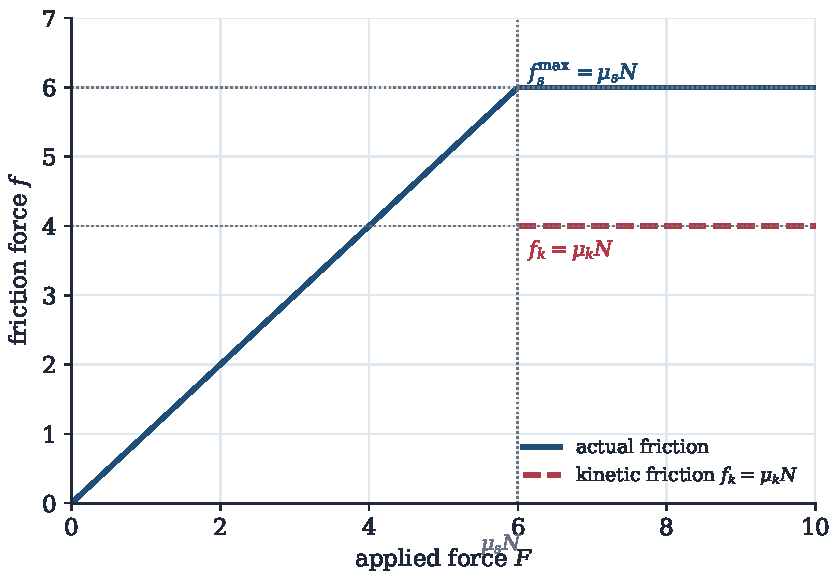
\includegraphics[width=0.78\textwidth]{figures/13_friction.pdf}
\caption{The friction force as a function of the applied force. The static
friction rises to $\mu_sN$; once sliding starts, the kinetic friction drops to
$\mu_kN$.}
\label{fig:friction}
\end{figure}

\begin{keyidea}[Angle of friction and angle of repose]
The maximum angle of an incline on which a body can rest without sliding is the
\emph{angle of repose}:
\[
\tan\alpha_c=\mu_s.
\]
For $\alpha<\alpha_c$, static friction can hold the body; for $\alpha>\alpha_c$,
it slides.
\end{keyidea}

\section{Rough inclined plane}

For a body sliding down a plane of angle $\alpha$ with kinetic friction,
\[
N=mg\cos\alpha,\qquad f_k=\mu_kN=\mu_kmg\cos\alpha,
\]
and along the plane
\[
ma=mg\sin\alpha-\mu_kmg\cos\alpha,
\]
so
\[
\boxed{a=g\left(\sin\alpha-\mu_k\cos\alpha\right).}
\]
If the body is pushed up the plane, friction reverses and
$a=-g(\sin\alpha+\mu_k\cos\alpha)$.

\section{Connected bodies and pulleys}

For an ideal (massless, frictionless) pulley, the tension is the same on both
sides of the string. The masses have the same magnitude of acceleration, possibly
in opposite directions. The method is always:
\begin{enumerate}[leftmargin=1.5em,itemsep=2pt]
  \item choose a positive direction of motion;
  \item write Newton's second law for each body separately;
  \item use the constraint (same string length) to relate accelerations;
  \item solve the resulting linear system.
\end{enumerate}

\begin{figure}[htbp]
\centering
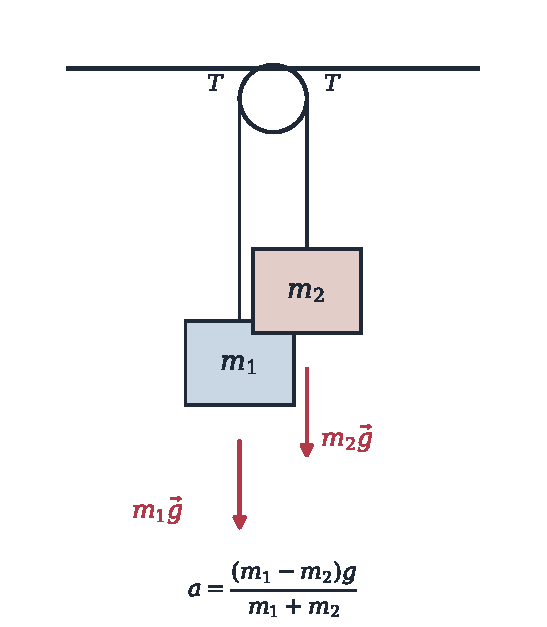
\includegraphics[width=0.52\textwidth]{figures/12_atwood.pdf}
\caption{The Atwood machine. The heavier mass descends; both masses have the same
magnitude of acceleration.}
\label{fig:atwood}
\end{figure}

\section{Elastic springs}

For an ideal spring of stiffness $k$ and natural length $l_0$,
\[
\vec F=-k(l-l_0)\,\vec u,
\]
where $\vec u$ points from the support to the free end. If $x=l-l_0$ is the
extension,
\[
F_x=-kx.
\]
At static equilibrium, the spring force balances the other forces.

\begin{figure}[htbp]
\centering
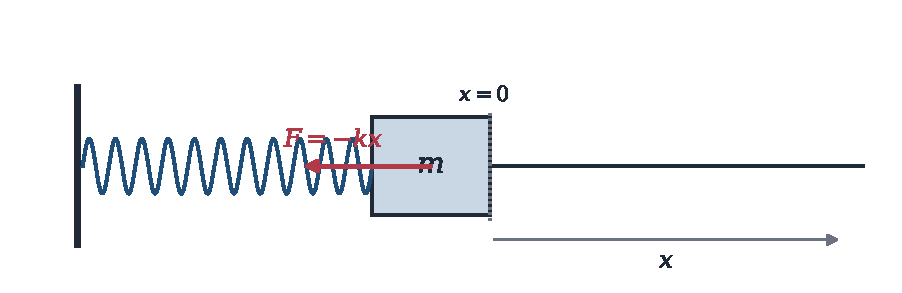
\includegraphics[width=0.82\textwidth]{figures/14_spring_mass.pdf}
\caption{A mass attached to a horizontal spring. The restoring force is
proportional to the displacement from equilibrium and points opposite to it.}
\label{fig:spring-mass}
\end{figure}

For springs in \textbf{series}, the same force acts on both and
\[
\frac1{k_{\mathrm{eq}}}=\frac1{k_1}+\frac1{k_2}.
\]
For springs in \textbf{parallel}, the extensions are equal and
\[
k_{\mathrm{eq}}=k_1+k_2.
\]

\section{Viscous drag and terminal velocity}

For slow motion in a fluid, a common model is
\[
\vec f=-k\vec v.
\]
A body falling from rest under gravity then obeys
\[
m\frac{\dd v}{\dd t}=mg-kv.
\]
The solution is
\[
v(t)=v_L\left(1-e^{-t/\tau}\right),
\qquad
v_L=\frac{mg}{k},\qquad
\tau=\frac mk.
\]
The velocity approaches the terminal velocity $v_L$ exponentially.

\begin{figure}[htbp]
\centering
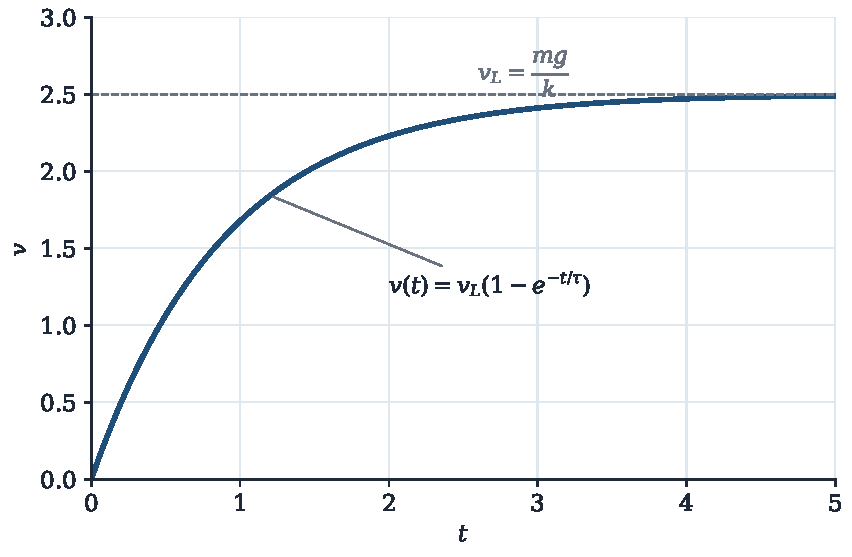
\includegraphics[width=0.72\textwidth]{figures/19_terminal_velocity.pdf}
\caption{Approach to terminal velocity for linear viscous drag.}
\label{fig:terminal}
\end{figure}

% ===========================================================================
\section{Worked examples}

\begin{worked}[Rough incline]
A block of mass $m=10.0\ \mathrm{kg}$ is placed on a plane inclined at
$\alpha=30.0^\circ$. The coefficients are $\mu_s=0.600$ and $\mu_k=0.250$.
(a) Does the block slide? (b) If it slides, find its acceleration.
\end{worked}

\begin{solution}{9.1}
The component of weight down the plane is
\[
mg\sin\alpha=10.0(9.81)\sin30.0^\circ=49.1\ \mathrm{N}.
\]
The normal reaction is
\[
N=mg\cos\alpha=10.0(9.81)\cos30.0^\circ=85.0\ \mathrm{N}.
\]
The maximum static friction is
\[
f_s^{\max}=\mu_sN=0.600(85.0)=51.0\ \mathrm{N}.
\]
Since $49.1<51.0$, the block does not slide.

If the block were already sliding, the kinetic friction would be
\[
f_k=\mu_kN=0.250(85.0)=21.3\ \mathrm{N},
\]
and the acceleration down the plane would be
\[
a=g(\sin\alpha-\mu_k\cos\alpha)
=9.81(0.500-0.250(0.866))=2.78\ \mathrm{m\,s^{-2}}.
\]
\end{solution}

\begin{worked}[Spring and mass]
A mass $m=0.500\ \mathrm{kg}$ is attached to a horizontal spring of stiffness
$k=200\ \mathrm{N\,m^{-1}}$ on a frictionless surface. The mass is pulled
$0.100\ \mathrm{m}$ from equilibrium and released.
(a) Find the spring force and acceleration at the instant of release.
(b) Find the acceleration when the mass passes through equilibrium.
\end{worked}

\begin{solution}{9.2}
(a) At release, $x=0.100\ \mathrm{m}$:
\[
F_x=-kx=-200(0.100)=-20.0\ \mathrm{N}.
\]
\[
a_x=\frac{F_x}{m}=\frac{-20.0}{0.500}=-40.0\ \mathrm{m\,s^{-2}}.
\]
The minus sign means the acceleration points back toward equilibrium.

(b) At equilibrium $x=0$, so $F_x=0$ and $a_x=0$. The velocity is maximum there.
\end{solution}

% ===========================================================================
\section{Exercises and Step-by-Step Solutions}

\begin{exercise}{\warm\ Starting a crate}
A crate of mass $50.0\ \mathrm{kg}$ rests on a horizontal floor. The coefficients
of friction are $\mu_s=0.500$ and $\mu_k=0.400$. Find the minimum horizontal force
needed to start the crate moving, and the force needed to keep it moving at
constant speed.
\end{exercise}

\begin{tabletworkspace}[6.5cm]
\end{tabletworkspace}

\begin{solution}{9.1}
\[
N=mg=50.0(9.81)=491\ \mathrm{N}.
\]
To start the motion:
\[
F_s=\mu_sN=0.500(491)=245\ \mathrm{N}.
\]
To keep it moving at constant speed:
\[
F_k=\mu_kN=0.400(491)=196\ \mathrm{N}.
\]
\end{solution}

\begin{exercise}{\warm\ Rough horizontal surface}
A $10.0\ \mathrm{kg}$ block is pulled horizontally by a force of
$50.0\ \mathrm{N}$ on a surface with $\mu_k=0.300$. Find its acceleration.
\end{exercise}

\begin{tabletworkspace}[6.5cm]
\end{tabletworkspace}

\begin{solution}{9.2}
\[
N=mg=10.0(9.81)=98.1\ \mathrm{N},\qquad
f_k=\mu_kN=0.300(98.1)=29.4\ \mathrm{N}.
\]
\[
a=\frac{F-f_k}{m}=\frac{50.0-29.4}{10.0}=2.06\ \mathrm{m\,s^{-2}}.
\]
\end{solution}

\begin{exercise}{\warm\ Spring extension}
A mass of $2.00\ \mathrm{kg}$ hangs from a vertical spring of stiffness
$k=300\ \mathrm{N\,m^{-1}}$. Find the extension at equilibrium and the force
needed to stretch the spring by $5.00\ \mathrm{cm}$.
\end{exercise}

\begin{tabletworkspace}[6.5cm]
\end{tabletworkspace}

\begin{solution}{9.3}
At equilibrium,
\[
kx=mg
\implies
x=\frac{mg}{k}=\frac{2.00(9.81)}{300}=0.0654\ \mathrm{m}.
\]
For a stretch $x=0.0500\ \mathrm{m}$,
\[
F=kx=300(0.0500)=15.0\ \mathrm{N}.
\]
\end{solution}

\begin{exercise}{\core\ Rough incline}
A block of mass $5.00\ \mathrm{kg}$ slides down a plane inclined at
$35.0^\circ$ with $\mu_k=0.200$. Find the normal reaction, the friction force,
and the acceleration.
\end{exercise}

\begin{tabletworkspace}[6.5cm]
\end{tabletworkspace}

\begin{solution}{9.4}
\[
N=mg\cos35.0^\circ=5.00(9.81)(0.8192)=40.2\ \mathrm{N}.
\]
\[
f_k=\mu_kN=0.200(40.2)=8.04\ \mathrm{N}.
\]
\[
a=g(\sin35.0^\circ-\mu_k\cos35.0^\circ)
=9.81(0.5736-0.1638)=4.02\ \mathrm{m\,s^{-2}}.
\]
\end{solution}

\begin{exercise}{\core\ Angle of repose}
The coefficient of static friction between a body and a plane is $\mu_s=0.450$.
Find the angle of repose. If the plane is inclined at $30.0^\circ$, does the body
slide?
\end{exercise}

\begin{tabletworkspace}[6.5cm]
\end{tabletworkspace}

\begin{solution}{9.5}
\[
\tan\alpha_c=\mu_s=0.450
\implies
\alpha_c=\arctan(0.450)=24.2^\circ.
\]
At $30.0^\circ>\alpha_c$, the body slides, because
$\tan30.0^\circ=0.577>0.450$.
\end{solution}

\begin{exercise}{\core\ Table, pulley, and friction}
A block $m_1=4.00\ \mathrm{kg}$ on a rough horizontal table
($\mu_k=0.250$) is connected by a string over a pulley to a hanging mass
$m_2=2.00\ \mathrm{kg}$. Find the acceleration and the tension.
\end{exercise}

\begin{tabletworkspace}[6.5cm]
\end{tabletworkspace}

\begin{solution}{9.6}
For $m_2$ (downward positive):
\[
m_2g-T=m_2a.
\]
For $m_1$:
\[
T-f_k=m_1a,\qquad f_k=\mu_km_1g.
\]
Adding,
\[
m_2g-\mu_km_1g=(m_1+m_2)a,
\]
\[
a=\frac{2.00(9.81)-0.250(4.00)(9.81)}{6.00}
=\frac{19.62-9.81}{6.00}=1.64\ \mathrm{m\,s^{-2}}.
\]
Then
\[
T=m_1(a+\mu_kg)=4.00(1.64+2.45)=16.4\ \mathrm{N}.
\]
\end{solution}

\begin{exercise}{\core\ Double incline}
Two masses $m_1=3.00\ \mathrm{kg}$ and $m_2=5.00\ \mathrm{kg}$ are connected by
a string over a pulley at the top of a double incline with angles
$\alpha=30.0^\circ$ for $m_1$ and $\beta=45.0^\circ$ for $m_2$. The surfaces are
frictionless. Find the acceleration and the tension.
\end{exercise}

\begin{tabletworkspace}[6.5cm]
\end{tabletworkspace}

\begin{solution}{9.7}
Assume $m_2$ slides down its plane and $m_1$ moves up its plane. For $m_1$:
\[
T-m_1g\sin\alpha=m_1a.
\]
For $m_2$:
\[
m_2g\sin\beta-T=m_2a.
\]
Adding,
\[
a=\frac{m_2g\sin\beta-m_1g\sin\alpha}{m_1+m_2}.
\]
\[
a=\frac{5.00(9.81)\sin45.0^\circ-3.00(9.81)\sin30.0^\circ}{8.00}
=\frac{34.68-14.72}{8.00}=2.50\ \mathrm{m\,s^{-2}}.
\]
\[
T=m_1(g\sin\alpha+a)=3.00(4.91+2.50)=22.2\ \mathrm{N}.
\]
\end{solution}

\begin{exercise}{\core\ Terminal velocity}
A body of mass $0.200\ \mathrm{kg}$ falls from rest subject to linear drag
$f=kv$ with $k=0.500\ \mathrm{kg\,s^{-1}}$. Find the terminal velocity, the time
constant, the speed at $t=1.20\ \mathrm{s}$, and the time to reach $99\%$ of the
terminal velocity.
\end{exercise}

\begin{tabletworkspace}[6.5cm]
\end{tabletworkspace}

\begin{solution}{9.8}
\[
v_L=\frac{mg}{k}=\frac{0.200(9.81)}{0.500}=3.92\ \mathrm{m\,s^{-1}},
\]
\[
\tau=\frac mk=\frac{0.200}{0.500}=0.400\ \mathrm{s}.
\]
At $t=1.20\ \mathrm{s}=3\tau$:
\[
v=3.92\left(1-e^{-3}\right)=3.92(0.950)=3.73\ \mathrm{m\,s^{-1}}.
\]
For $99\%$ of terminal velocity,
\[
1-e^{-t/\tau}=0.99
\implies
e^{-t/\tau}=0.01
\implies
t=\tau\ln100=0.400(4.605)=1.84\ \mathrm{s}.
\]
\end{solution}

\begin{exercise}{\mastery\ Springs in series and parallel}
Two springs of stiffness $k_1=100\ \mathrm{N\,m^{-1}}$ and
$k_2=200\ \mathrm{N\,m^{-1}}$ are combined. Find the equivalent stiffness
(a) in series and (b) in parallel. A mass of $2.00\ \mathrm{kg}$ hangs from each
combination; find the equilibrium extension in each case.
\end{exercise}

\begin{tabletworkspace}[6.5cm]
\end{tabletworkspace}

\begin{solution}{9.9}
(a) Series:
\[
\frac1{k_{\mathrm{eq}}}=\frac1{100}+\frac1{200}
=\frac{3}{200}
\implies
k_{\mathrm{eq}}=66.7\ \mathrm{N\,m^{-1}}.
\]
The extension under $m=2.00\ \mathrm{kg}$:
\[
x=\frac{mg}{k_{\mathrm{eq}}}=\frac{19.62}{66.7}=0.294\ \mathrm{m}.
\]

(b) Parallel:
\[
k_{\mathrm{eq}}=100+200=300\ \mathrm{N\,m^{-1}},
\]
\[
x=\frac{19.62}{300}=0.0654\ \mathrm{m}.
\]
\end{solution}

\begin{exercise}{\mastery\ Optimal pulling angle}
A block of mass $m$ is pulled on a rough horizontal floor by a force $F$ making
an angle $\theta$ above the horizontal. The coefficient of kinetic friction is
$\mu_k$.
(a) Show that
\[
a=\frac Fm(\cos\theta+\mu_k\sin\theta)-\mu_kg.
\]
(b) Show that the acceleration is maximum when $\tan\theta=\mu_k$.
(c) For $m=10.0\ \mathrm{kg}$, $F=50.0\ \mathrm{N}$, and $\mu_k=0.300$, compute
the optimal angle and the maximum acceleration.
\end{exercise}

\begin{tabletworkspace}[6.5cm]
\end{tabletworkspace}

\begin{solution}{9.10}
(a) The normal reaction is reduced by the vertical component of the pull:
\[
N=mg-F\sin\theta.
\]
The friction is $f_k=\mu_kN$, and the horizontal equation is
\[
ma=F\cos\theta-f_k=F\cos\theta-\mu_k(mg-F\sin\theta).
\]
Dividing by $m$,
\[
a=\frac Fm(\cos\theta+\mu_k\sin\theta)-\mu_kg.
\]

(b) Differentiate with respect to $\theta$:
\[
\frac{\dd a}{\dd\theta}=\frac Fm(-\sin\theta+\mu_k\cos\theta).
\]
Setting this to zero gives
\[
\tan\theta=\mu_k.
\]
The second derivative is negative at this point, so it is a maximum.

(c)
\[
\theta=\arctan(0.300)=16.7^\circ.
\]
\[
a_{\max}=\frac{50.0}{10.0}\left(\cos16.7^\circ+0.300\sin16.7^\circ\right)
-0.300(9.81).
\]
\[
a_{\max}=5.00(0.9578+0.0862)-2.943=5.22-2.94=2.28\ \mathrm{m\,s^{-2}}.
\]
\end{solution}

